\documentclass{beamer}
\usepackage{lmodern}
\usepackage{pdfpages}
\usetheme{ITU}

\title{Distributed DCR in a TEE}
\author{Malthe Kirkbro, Mikkel Gaub, Frederik Madsen}
\date{January 17, 2018}

\begin{document}
\setbeamertemplate{caption}{\raggedright\insertcaption\par}


	\begin{frame}
		\maketitle
	\end{frame}

	\begin{frame}{The Problem} %Frederik
		\begin{itemize}
			\item Create a Distributed DCR engine
			\begin{itemize}
				\item Consensus
				\item SGX
			\end{itemize}
		\end{itemize}
	\end{frame}

	\begin{frame}{SGX} %Frederik
		\begin{itemize}
			\item Trusted Execution Environment
			\begin{itemize}
				\item Integrity
				\item Confidentiality
			\end{itemize}
			\item Obtained via secret fused onto the CPU. Examples:
			\begin{itemize}
				\item Sealing secret (during manufacturing)
				\item Provisioning secret (after manufacturing)
			\end{itemize}
		\end{itemize}
	\end{frame}

	\begin{frame}{Enclave} %Malthe
		\begin{itemize}
			\item Processor Reserved Memory (PRM)
			\item Enclave mode
			\item Enclave Page Cache (EPC)
		\end{itemize}
		\begin{itemize}
			\item SGX Enclave Control Structure (SECS)
			\item Signature
		\end{itemize}
	\end{frame}

	\begin{frame}{EGETKEY}
		\includepdf[pages=81,viewport=300 290 570 600, clip, scale=.75]{sgx-explained.pdf}

		\vspace{\stretch{100}}\center\fontsize{4pt}{1}\selectfont
		Victor Costan \& Srinivas Devadas. Intel SGX Explained. IACR Cryptology ePrint Archive (2016)
	\end{frame}

	\begin{frame}{Attestation} %Malthe
		\begin{itemize}
			\item Local
				\begin{itemize}
					\item Report MACed with CPU-fused key (EREPORT)
				\end{itemize}
			\item Remote
				\begin{itemize}
					\item Locally attested report signed by EPID private key
				\end{itemize}
		\end{itemize}
	\end{frame}

	\begin{frame}{EREPORT}
		\includepdf[pages=84,viewport=25 160 300 575, clip, scale=.75]{sgx-explained.pdf}

		\vspace{\stretch{100}}\center\fontsize{4pt}{1}\selectfont
		Victor Costan \& Srinivas Devadas. Intel SGX Explained. IACR Cryptology ePrint Archive (2016)
	\end{frame}

	\begin{frame}{Trusted Monotonic Counter} %Frederik
		\begin{itemize}
			\item Monotonic non-volatile counter
			\item Demo!
		\end{itemize}
	\end{frame}

	\begin{frame}{Security}	%Mikkel
		\begin{itemize}
			\item Attacks on confidentiality (including SPECTRE!)
			\begin{itemize}
				\item Note that this can be problematic with TLS keys after attestation
			\end{itemize}
			\item No (to us known) attacks on integrity
		\end{itemize}
	\end{frame}

	\begin{frame}{Related Works} %Mikkel
		\begin{itemize}
			\item Some solutions to similar problems exist, using SGX
		\end{itemize}
	\end{frame}

	\begin{frame}{FastBFT} %Mikkel
		\begin{itemize}
			\item BFT in \textit{O(n)} messages
			\item Distributing parts of a secret
			\item Vote numbering
		\end{itemize}
	\end{frame}

	\begin{frame}{Hyperledger Sawtooth}	%Mikkel
		\begin{itemize}
			\item Blockchain without mining
			\item PoET sent as evidence of block validity
		\end{itemize}
	\end{frame}

\end{document}